\appendix
\numberwithin{equation}{section}

\section{Supplementary monojet analysis}
\label{sec:monojet_method}

\subsection{Grid, production, and reconstructed signal}
\label{sec:monojet_grid}

The supplementary CMS EXO-20-004 recast uses a separate rate-matched grid with $72\le M_V\le200$ GeV, $20\le m_\chi\le100$ GeV, $0.10\le g_\chi\le1.50$, and $0.1\le g_t\le\sqrt{4\pi}$. Its recoil calculation uses a two-parameter Fermi density, $d_\gamma(0)=0$, and the finite spacelike $c,b,t$ photon-mixing contribution. It searches each side of the invisible threshold and assigns an on-shell template only where a unique root meets the narrow-width requirements. The 1015 coordinates yield 434 retained central-abundance on-shell solutions. This is a different slice from the primary top-pair grid.

The hard signal includes tree-level $q\bar q\to gV$ and $qg\to qV$ channels and their charge conjugates, plus the finite heavy-quark-loop channel $gg\to gV$. The three-point pure-vector $gg\to V$ amplitude cancels. We calculate the distinct initial states separately with MadGraph5\_aMC@NLO 3.6.6 and \texttt{nn23lo1} at 13 TeV and sum their rates. The loop UFO includes the rational $gggV$ term obtained from \texttt{loop\_sm}, with coefficient $i g_{Vq}g_s^3/(48\pi^2)$ per flavor and color structure $d^{abc}$. Its Ward/BRS test ratio is about $6.3\times10^{-24}$ at the tested 87.18 GeV mediator point and 1 TeV partonic energy. \cite{alwall2014,hirschi2015,cox2016}

On-shell production is normalized as $\sigma_X=\sigma_X^{\rm prod}(g_t=1)g_t^2\mathrm{BR}(V\to\chi_1\chi_2)$. Pythia 8.312 and Delphes 3.5.0 treat the mediator as invisible. Nominal samples start at generator $p_T^j=100$ GeV, with additional tree and loop samples above 350 and 480 GeV, respectively, combined in mutually exclusive intervals. The 120 GeV loop node also uses a 230 GeV boundary. Reconstructed cuts require a leading AK4 jet with $p_T>100$ GeV and $|\eta|<2.4$, $p_T^{\rm miss}>250$ GeV, jet azimuthal cuts, and lepton, photon, and heavy-flavor-related vetoes, including the 2018 HEM treatment. The 2016--2018 data contain 22 bins per year and about $137\ \mathrm{fb}^{-1}$. \cite{pythia2022,delphes2014,cmsmonojet,albert2021}

\subsection{Likelihood and central limits}
\label{sec:monojet_results}

The public control-region background prediction and covariance, observed counts, and simulated signal define

\begin{equation}
\label{eq:likelihood}
\begin{aligned}
\mathcal L(\mu,\mathbf b',\mathbf s') &=
\prod_{i=1}^{66}\operatorname{Pois}(n_i\mid b_i'+\mu s_i')\\
&\quad\times G(\mathbf b';\mathbf b,C_b)\,G(\mathbf s';\mathbf s,C_s).
\end{aligned}
\end{equation}

The signal covariance contains finite-template counting correlations, integration errors, and a common 1.6\% luminosity uncertainty, retaining correlations across years that share events. Yields are linearly interpolated in mass and independent covariances combined with squared weights. We profile nonnegative signal yields and positive Poisson means and solve asymptotic $CL_s=0.05$. Expected limits use a background Asimov data set, and observed limits use the measured counts with a conditional background Asimov construction. \cite{cmscovariance,cmsyields,cmssimplified,cowan2011,read2002}

Reference templates give 208 expected and 151 observed sampled points with $\mu_{95}<1$; the lowest sampled mediator masses are 92 and 104 GeV. The smallest observed reference-template limit is 0.181 at $(M_V,g_t)=(200\,\mathrm{GeV},\sqrt{4\pi})$. The following three reference benchmarks remain below unity under the prescribed yield variations.

\begin{table*}[tbp]
\caption{Supplementary monojet benchmarks and their reference-template limits.}
\label{tab:benchmarks}
\begin{ruledtabular}
\begin{tabular}{rrrrr}
$M_V$ [GeV] & $g_t$ & Expected $\mu_{95}$ & Observed $\mu_{95}$ & Observed, $r=0.75$--$1.25$ \\
\hline
120 & 3.073 & 0.412 & 0.607 & 0.570--0.664 \\
150.4 & 3.545 & 0.184 & 0.340 & 0.329--0.357 \\
190.4 & 3.545 & 0.219 & 0.273 & 0.270--0.277 \\
\end{tabular}
\end{ruledtabular}
\end{table*}

\begin{figure*}[tbp]
\centering
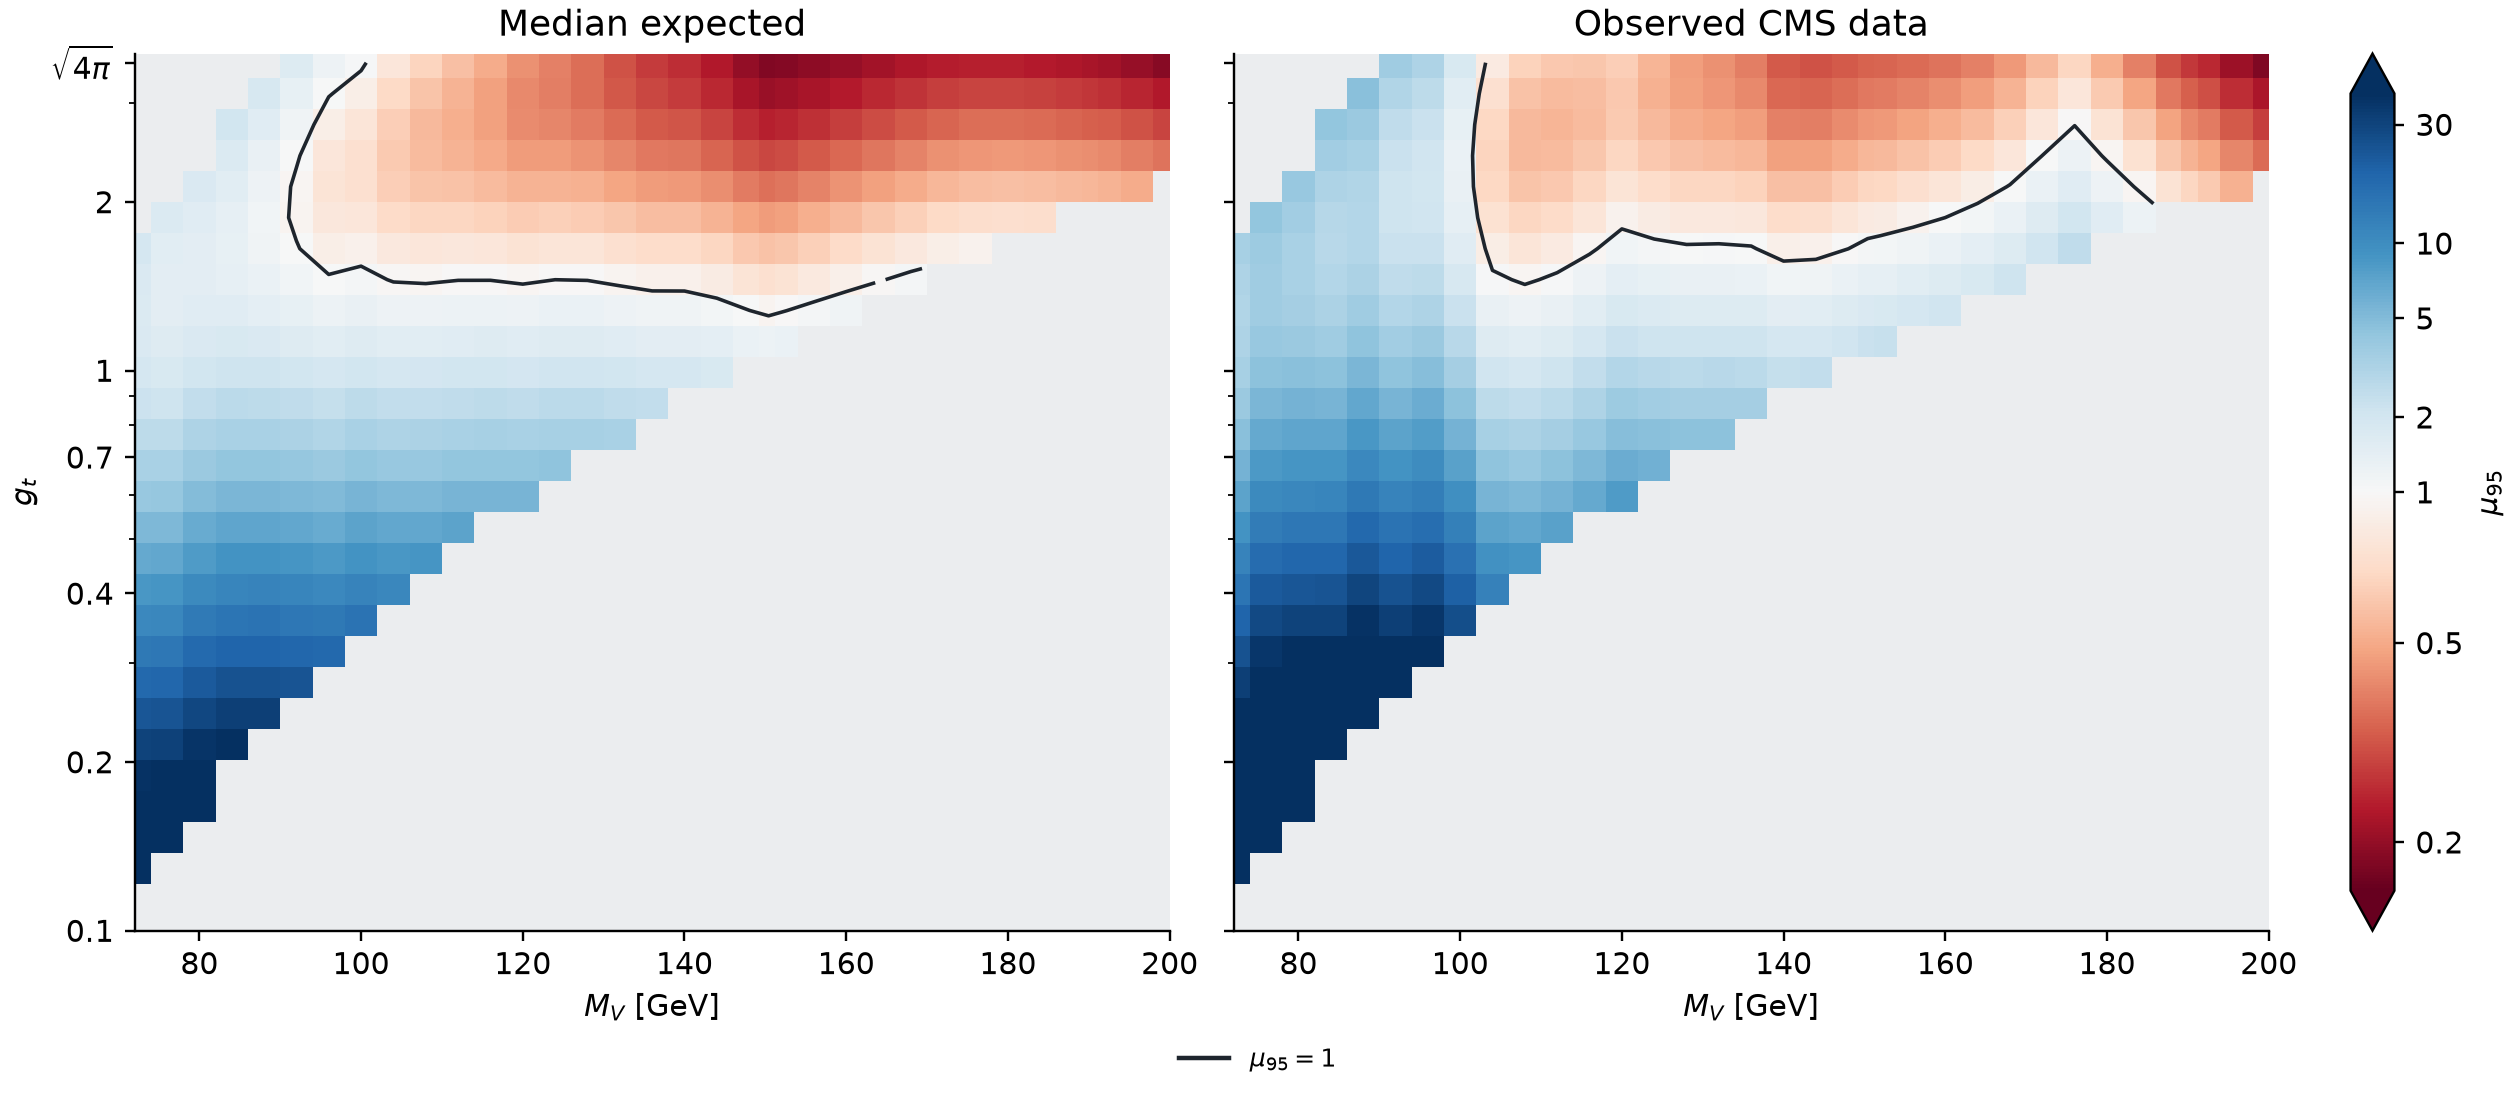
\includegraphics[width=\linewidth]{figures/04_cms_central_plane.png}
\caption{Expected and observed CMS monojet 95\% confidence-level limits on the unique branch satisfying the recoil-yield, central-abundance, and narrow-width conditions. The black contour marks $\mu_{95}=1$. Gray denotes coordinates with no unique in-scope solution.}
\label{fig:exclusion}
\end{figure*}

At the representative points tested, changing the Planck target by $\pm2\sigma$ changes the median expected limit by at most 0.44\%. The yield test $r=0.75$--1.25 changes it by at most 9.4\%; reducing $f_2$ to 0.45 or 0.30 changes it by up to 3.0\% or 12.8\%. The tested $|d_\gamma(0)|\le7\times10^{-6}$ variation changes it by at most 2.8\%. These are monojet checks on its own grid, not uncertainty estimates for the primary top-pair map. At $r=2$, the three benchmark observed limits remain below unity at 0.507, 0.310, and 0.265. A lower-coupling 150.4 GeV point remains above unity, and some low-abundance roots disappear at the dark-coupling scan boundary.

\subsection{Official benchmark and template validation}
\label{sec:validation}

Using official CMS vector templates, the reconstructed expected and observed mediator mass boundaries are 2.208 and 1.941 TeV, compared with official values of 2.198 and 1.957 TeV. Individual observed limits disagree more at low mass. This checks the statistical reconstruction using official templates. \cite{cmsmonojet,cmssignal}

\begin{figure*}[tbp]
\centering
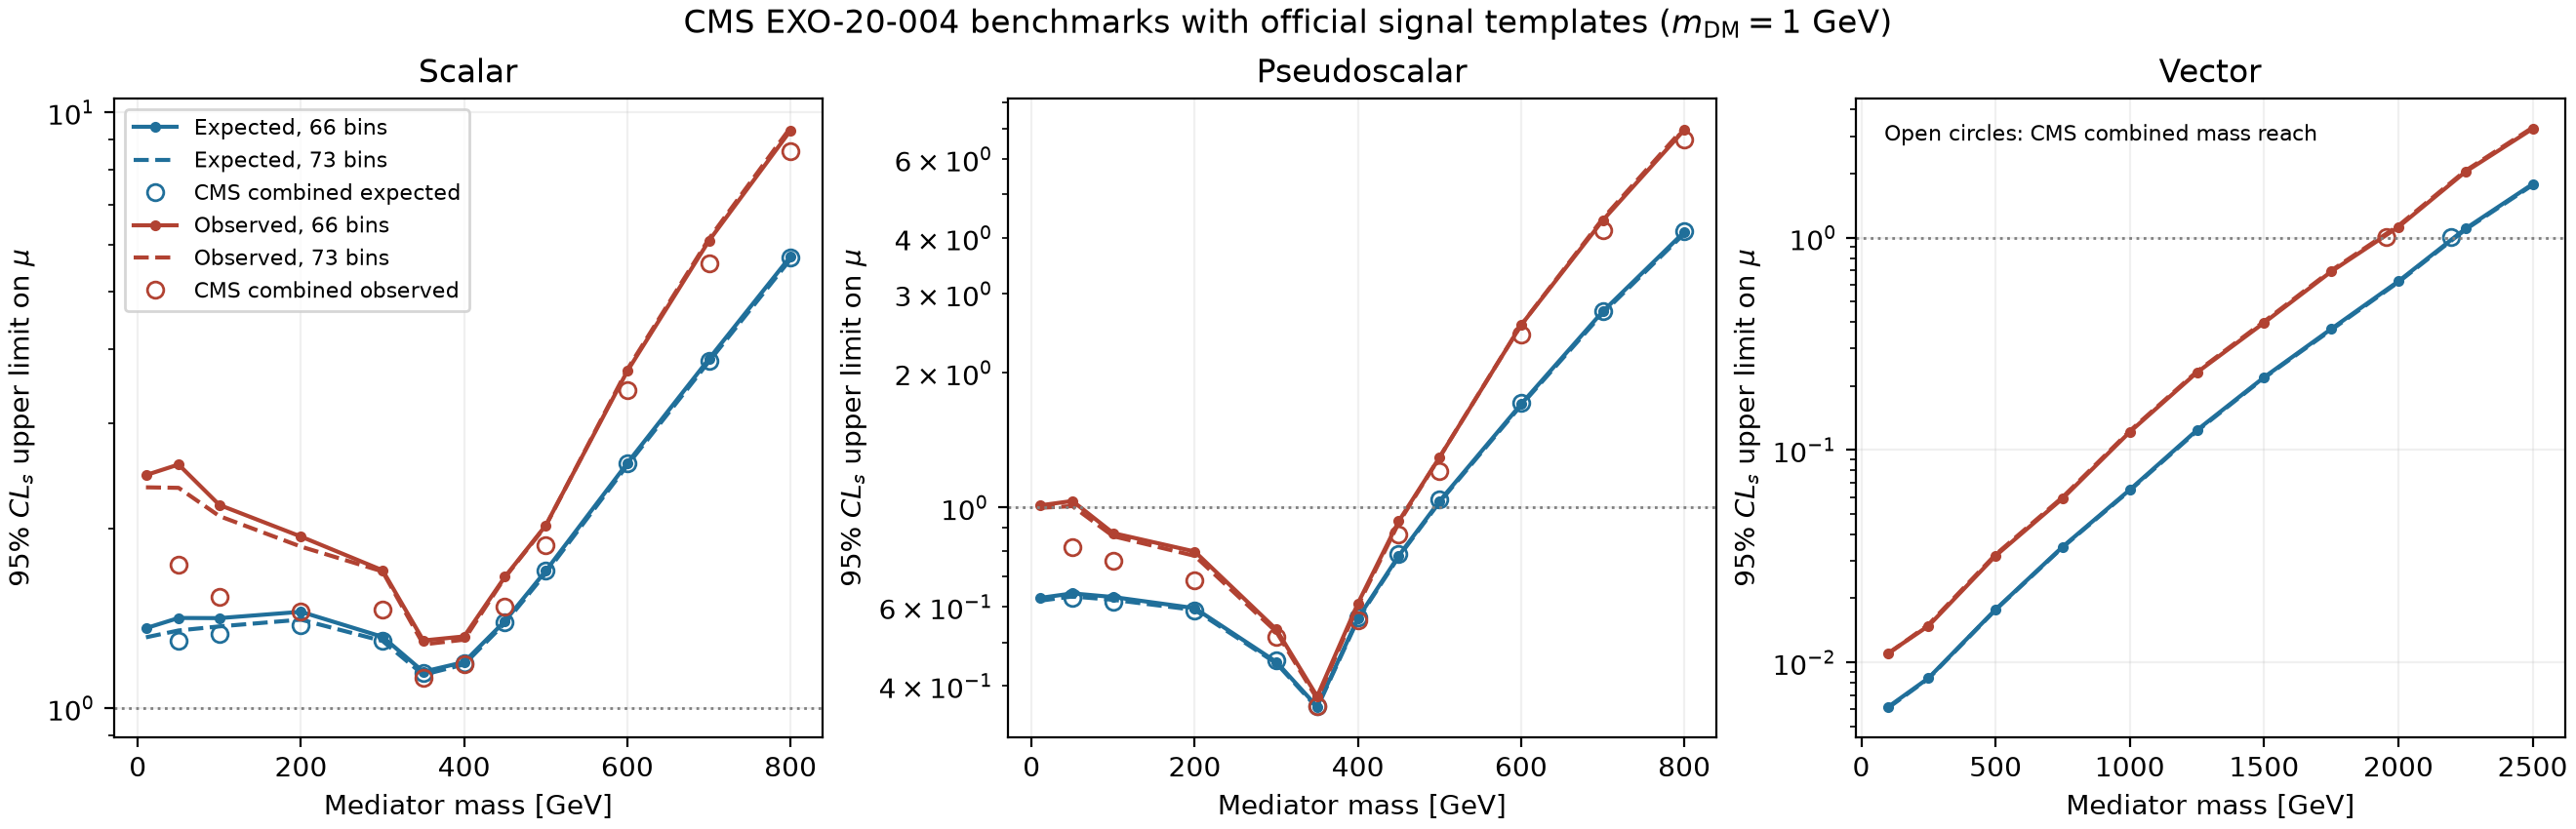
\includegraphics[width=\linewidth]{figures/c01_cms_benchmark_limits.png}
\caption{Comparison of limits obtained using official CMS signal templates. For scalar and pseudoscalar benchmarks between 50 and 800 GeV, the expected limits from the 66-bin fit differ from the published combination by at most about $9\%$. The largest difference in observed limits is about $48\%$. The mass boundaries provide a separate check of the overall reach for the official vector benchmark. \cite{cmsmonojet,cmssignal}}
\label{fig:cms_official}
\end{figure*}

Independent LO plus Delphes simulation gives 62.9\% of the official 2017 100 GeV vector signal yield. The independent and official samples differ in generation and reconstruction settings. The discrepancy limits validation of absolute acceptance, including heavy-flavor-related selections, and remains relevant to the inferred exclusion boundary.

\begin{figure*}[tbp]
\centering
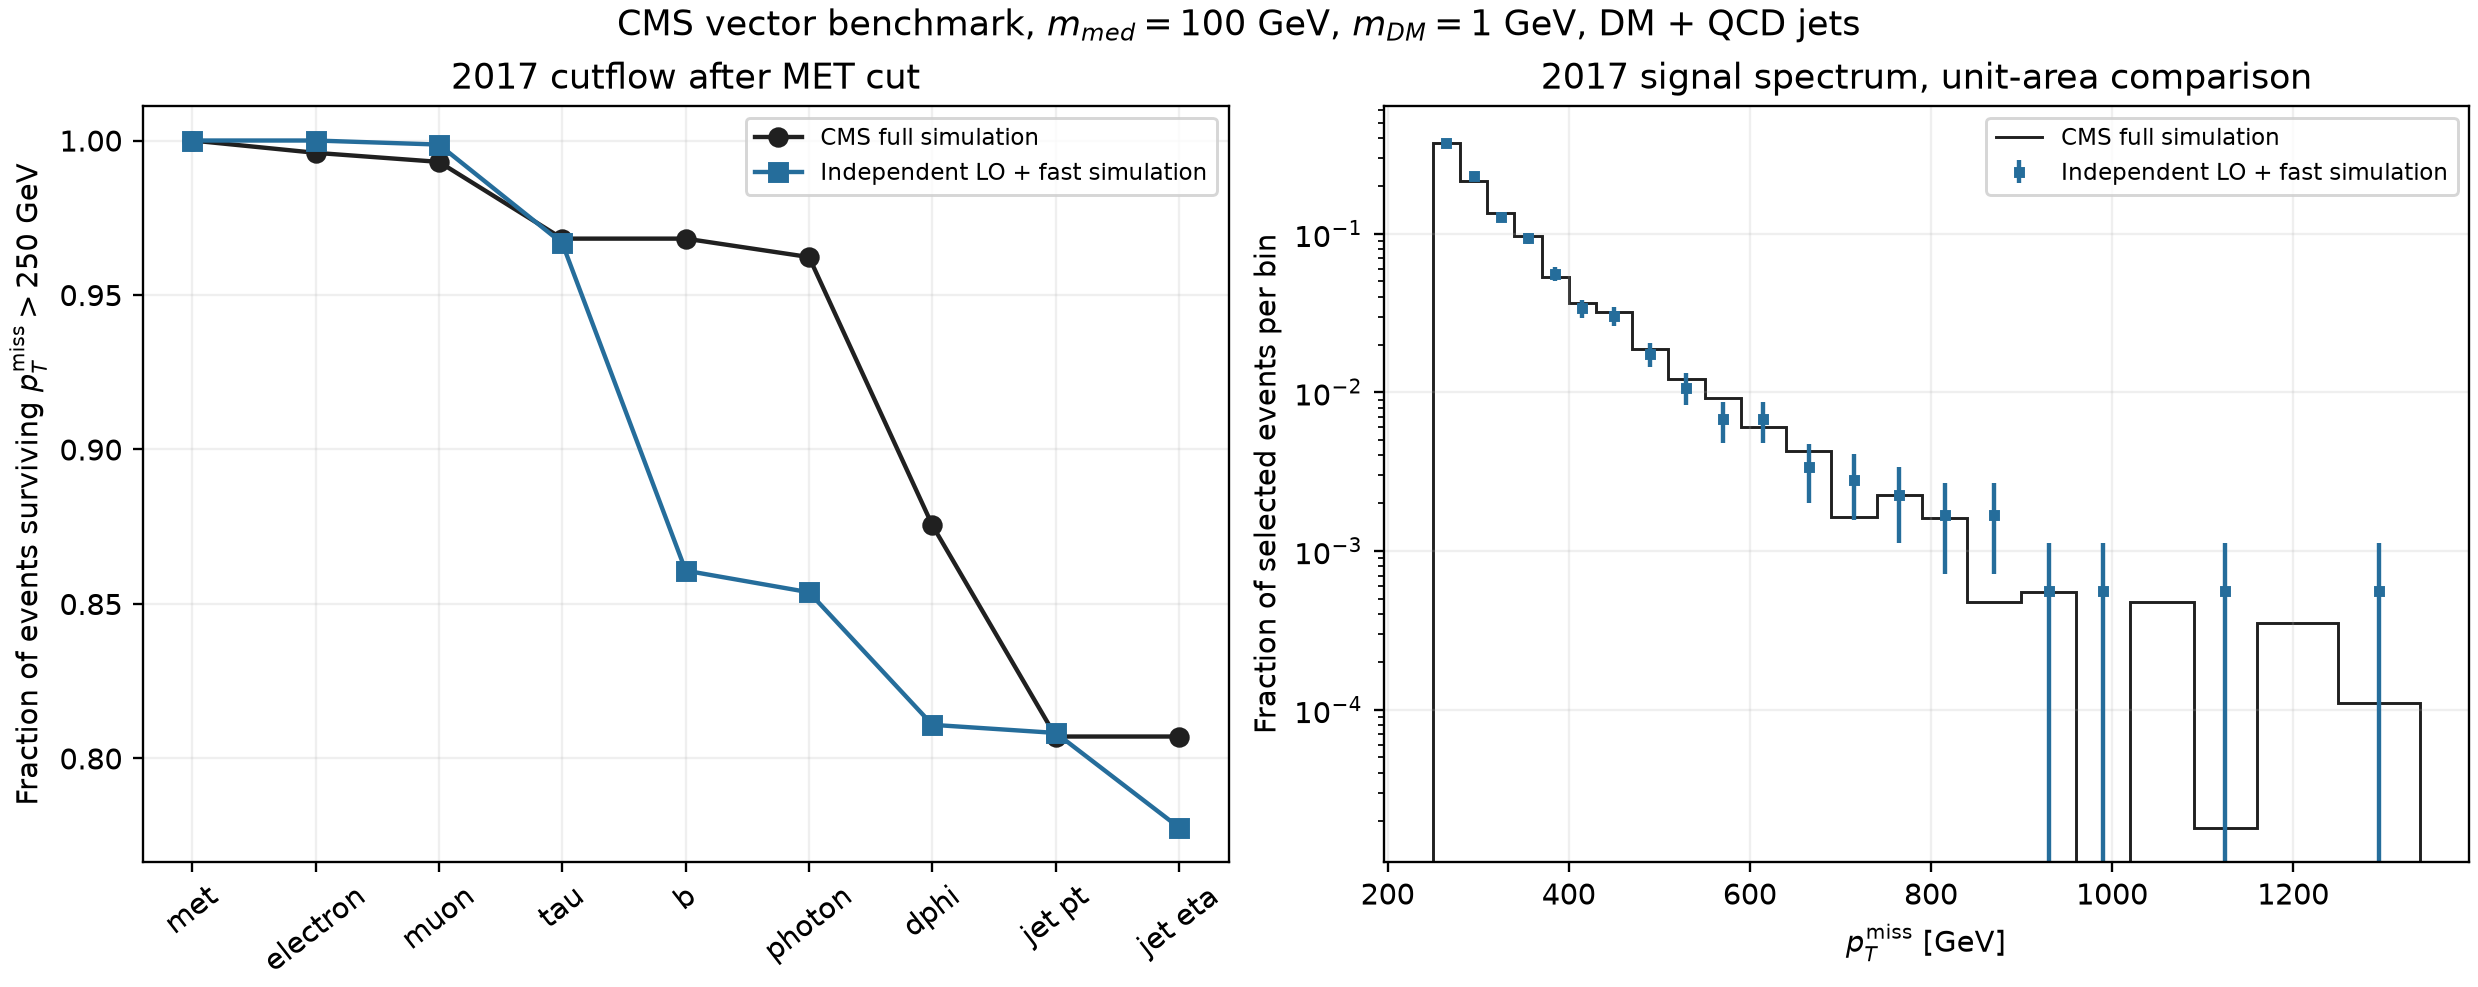
\includegraphics[width=\linewidth]{figures/c03_cms_vector_100.png}
\caption{Cutflow and MET spectrum for the 100 GeV CMS vector benchmark. Comparison of independent LO event generation and fast detector simulation with official CMS vector benchmarks. For the 100 GeV benchmark in 2017, the efficiency after the MET cut is $76.91\%$ for CMS and $77.76\%$ in our simulation. The absolute QCD signal yield in our simulation is 0.629 times the CMS yield. The two samples use different generator and reconstruction settings, including NLO matching in the official sample. We compare the normalized shapes and the absolute yields separately. \cite{cmscutflow}}
\label{fig:cms_100}
\end{figure*}

Independent loop replicas and stratified tail samples test three sensitive nodes. The templates agree within about 1.7 Monte Carlo standard deviations in the key bins and combined high-MET intervals. Across the tested templates and yield targets, all three exclusion decisions persist, with a largest observed limit of 0.680. However, pooled-template limits at 150.4 and 190.4 GeV are about 31\% and 27\% below the reference values, respectively. Replacing the relevant mass templates changes the full-grid counts to 199 expected and 162 observed sampled points below unity, while the lowest sampled masses remain 92 and 104 GeV. Finite-template and acceptance effects therefore remain material to numerical contours.

\begin{figure*}[tbp]
\centering
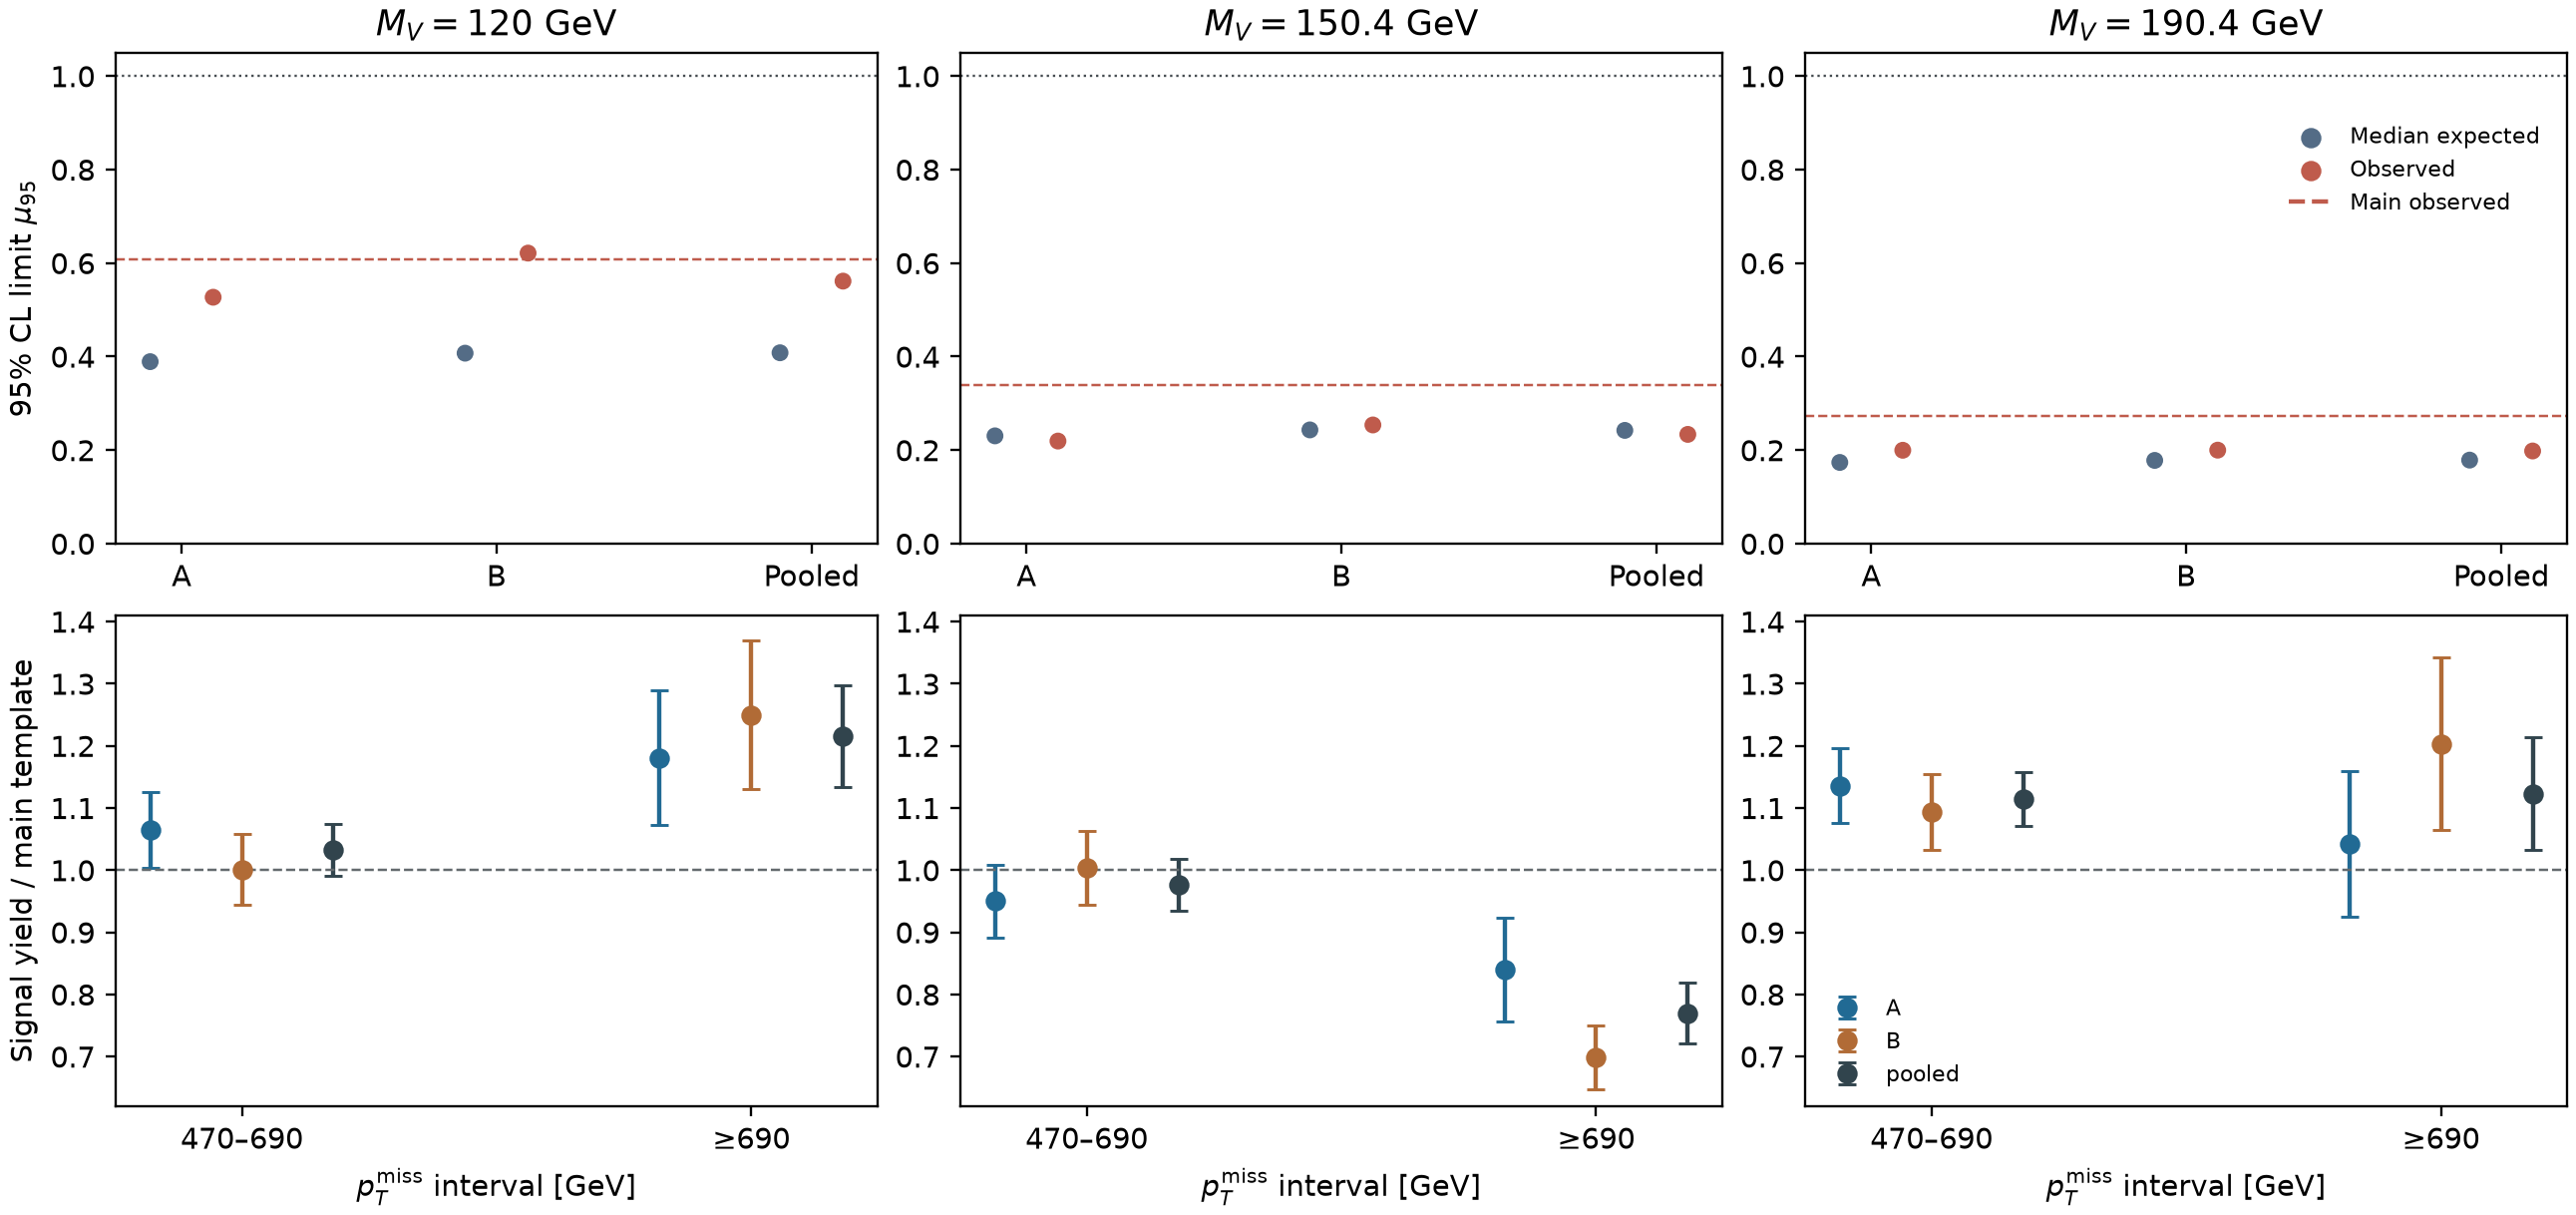
\includegraphics[width=\linewidth]{figures/c06_three_template_replicas.png}
\caption{Independent loop-template replicas and pooled templates at the three sensitive monojet benchmarks. The upper panels compare the fitted limits. The lower panels compare yields in the combined MET intervals, with Monte Carlo uncertainty bars.}
\label{fig:independent_samples}
\end{figure*}

\section{Recoil matching and late-state assumptions}
\label{sec:matching}

\subsection{Photon matching}
\label{sec:low_energy}

Photon kinetic mixing adds an electromagnetic-current coupling. We define $d_\gamma=e\epsilon_\gamma/g_t$; its zero-momentum value is an independent matching input. Relative to zero momentum, the retained heavy-quark term is

\begin{equation}
\label{eq:finite_mixing}
\begin{aligned}
\delta d_{cbt}(s)&=-\frac{2\alpha}{\pi}\sum_{q=c,b,t}N_cQ_q\frac{\widehat m_q}{m_t}\\
&\quad\times\int_0^1 dx\,x(1-x)\log\left[1-\frac{s x(1-x)}{\widehat m_q^2}-i0\right].
\end{aligned}
\end{equation}

With a common Helm form factor, the nuclear charge shifts by $g_tZ[d_\gamma(0)+\delta d_{cbt}(-q^2)]$. For $^{131}$Xe, $Q_A/g_t\simeq8.05\times10^{-3}$, so cancellation occurs near $d_\gamma(0)=-1.49\times10^{-4}$. At 35 GeV and zero matching input, the retained finite spacelike term reduces the integrated rate by about 0.077\%. Varying the matching input to $\mp7\times10^{-6}$ changes the fixed-coupling rate to 0.908 or 1.095 times the tree result, requiring $\kappa/\kappa_0=1.050$ or 0.956. Near cancellation this ratio reaches about 56.5. These matching checks motivate stating the prescription separately for the two collider grids. \cite{deramo2016,forner2026}

\begin{figure*}[tbp]
\centering
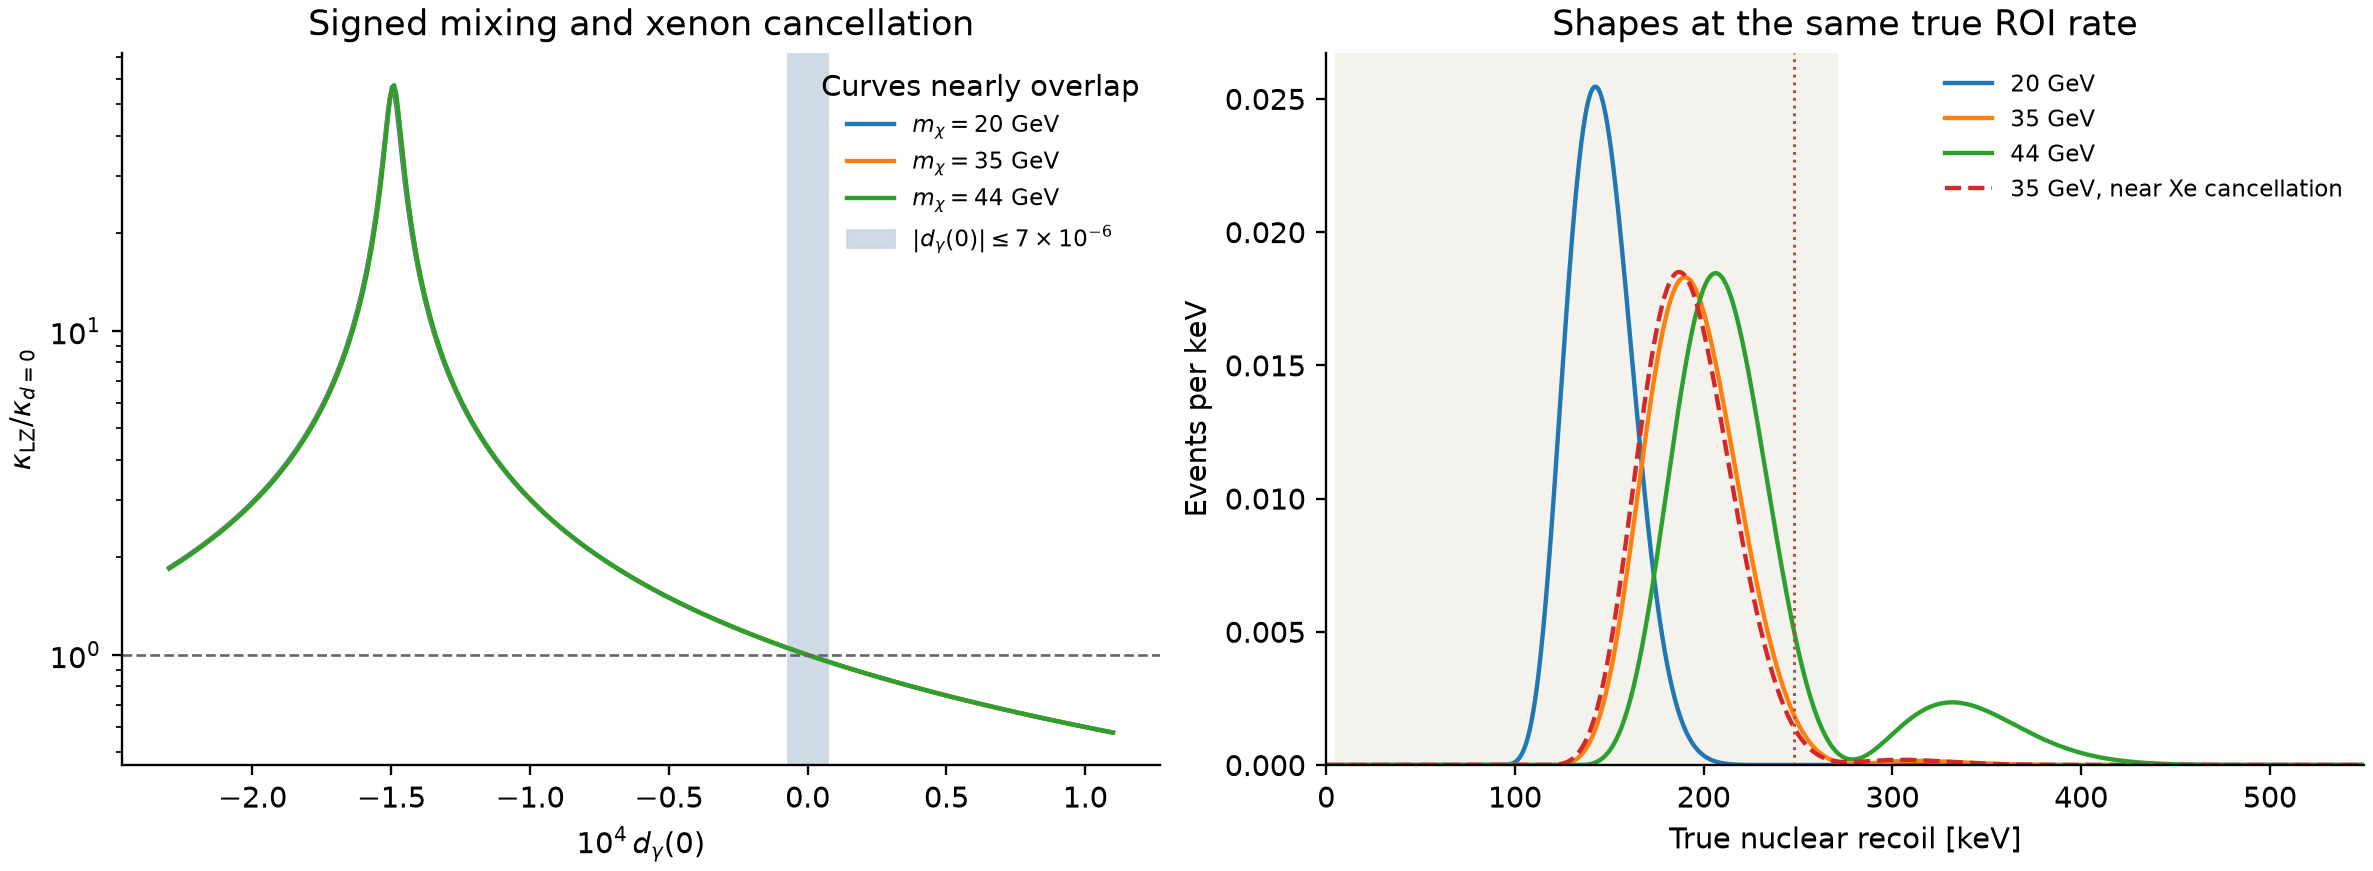
\includegraphics[width=\linewidth]{figures/06_matching_and_spectra.png}
\caption{The left panel shows how photon mixing changes the coupling required to match the yield. The right panel compares spectra with the same integrated truth-level yield. After Gaussian smoothing with a width of 32.5 keV, the signal densities near 248 keV at $m_\chi=20,35,44$ GeV are approximately $2.75\times10^{-4}$, $4.54\times10^{-3}$, and $6.98\times10^{-3}$ events/keV. The energy-spectrum approximation uses Gaussian smoothing alone. The LZ S1/S2 response and backgrounds enter an event-level analysis.}
\label{fig:mixing}
\end{figure*}

\subsection{Present excited fraction}

The main scan fixes $f_2=0.5$. After freeze-out, conversion is modeled by

\begin{equation}
\dot f_2=-n_\chi\langle\sigma v\rangle_{22\to11}
[f_2^2-e^{-2\Delta m/T_\chi}(1-f_2)^2].
\end{equation}

Born contact-scattering estimates with varied kinetic-decoupling assumptions give a minimum near 0.45 at the tested on-shell benchmarks and about 0.30 at some off-shell benchmarks, assuming additional decay is suppressed. The 1 MeV splitting closes the electron-pair decay channel; independent $V$--$Z$ mixing or a transition dipole can alter the excited-state lifetime. These calculations define thermal-history benchmarks, not a determination of $f_2$ across the full top-pair grid. The top-pair abundance-endpoint tests keep $f_2$ fixed. \cite{gemmell2026,carrillo2022}

\begin{figure*}[tbp]
\centering
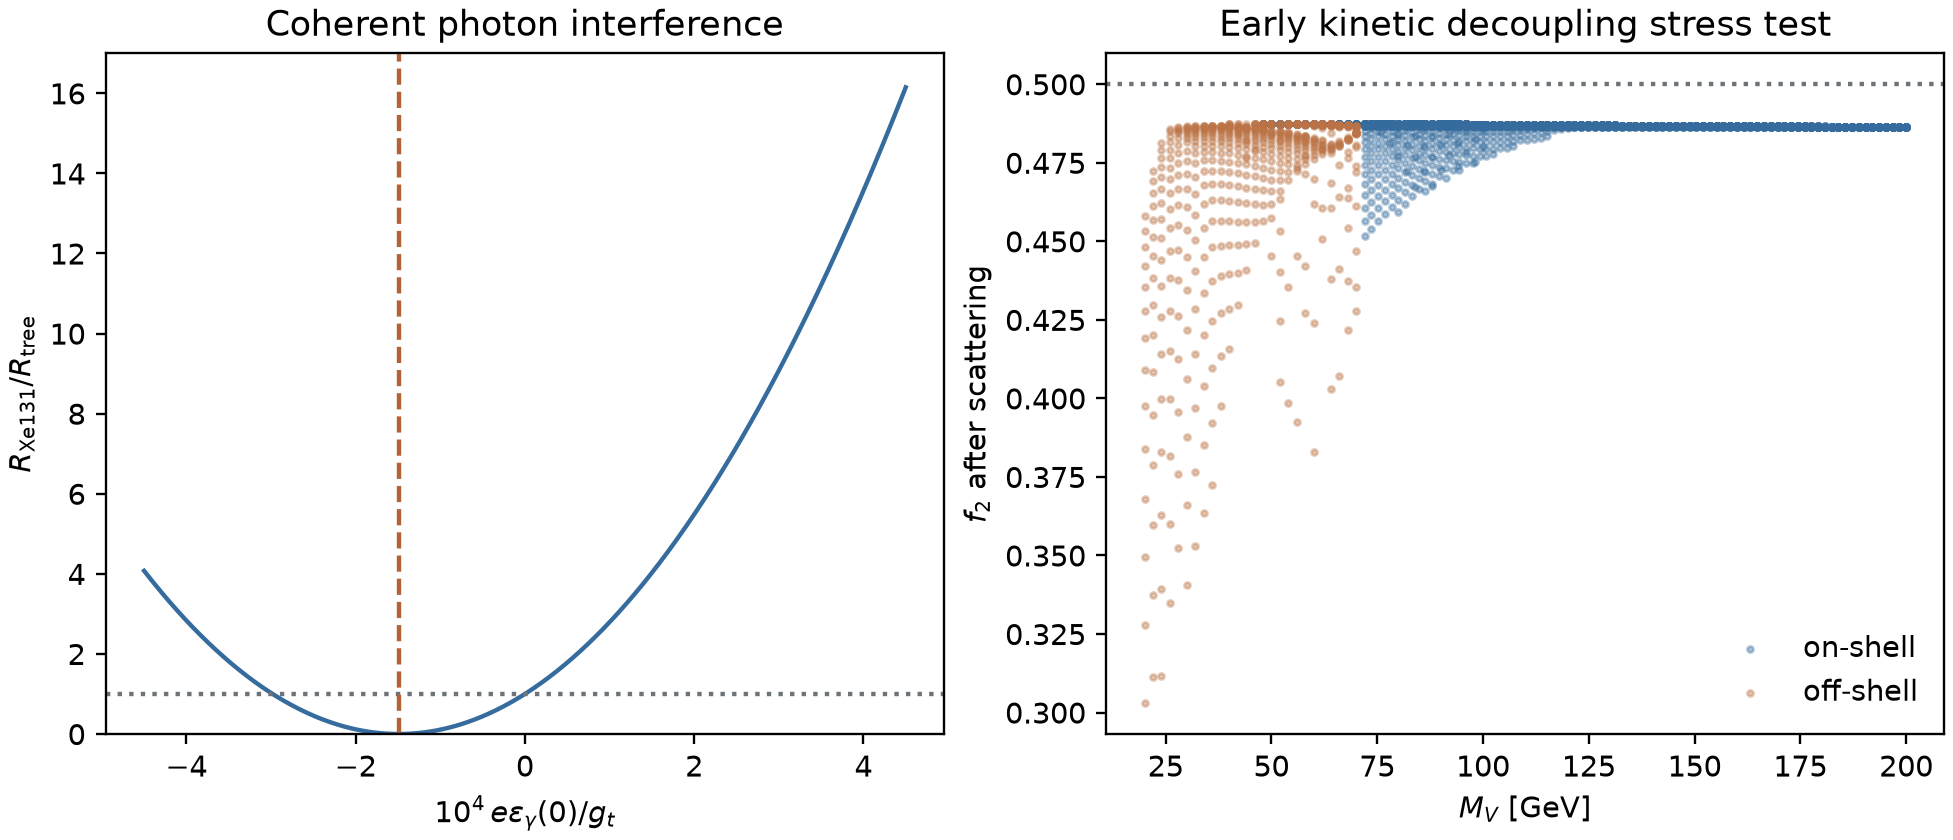
\includegraphics[width=\linewidth]{figures/a03_excited_fraction.png}
\caption{The conversion $\chi_2\chi_2\leftrightarrow\chi_1\chi_1$ can change the excited-state fraction after chemical freeze-out. In the standard thermal histories tested, with additional decay suppressed and the Standard Model bath included, the minimum at the on-shell benchmarks is $f_2\simeq0.45$ and falls to about $0.30$ at some off-shell benchmarks. The splitting $\Delta m<2m_e$ closes the electron-pair decay channel. Independent $V$--$Z$ mixing or a transition dipole can still affect the lifetime. \cite{gemmell2026,carrillo2022}}
\label{fig:fraction}
\end{figure*}

\section{Off-shell and single-top checks}
\label{sec:top}

At the same $(M_V,g_t)$, the yield and abundance equations can admit more than one dark mass. In a low-mass scan, $(M_V,g_t)=(48\,\mathrm{GeV},0.252)$ has central-abundance roots at 20.445, 25.260, and 45.878 GeV; the lightest is on shell. The primary top-pair map retains only its defined on-shell branch. Below the invisible threshold, production must be calculated with the full four-body amplitude rather than an on-shell rate times a branching fraction.

At three off-shell benchmarks with mediator masses 30, 46, and 60 GeV, full matrix elements with truth $p_T^{\rm miss}>250$ GeV give top-pair cross sections of 0.033, 0.041, and 1.13 fb. These truth-level rates do not define an off-shell exclusion; top decays, reconstruction, and an appropriate likelihood would be needed. \cite{cmstop}

\begin{figure*}[tbp]
\centering
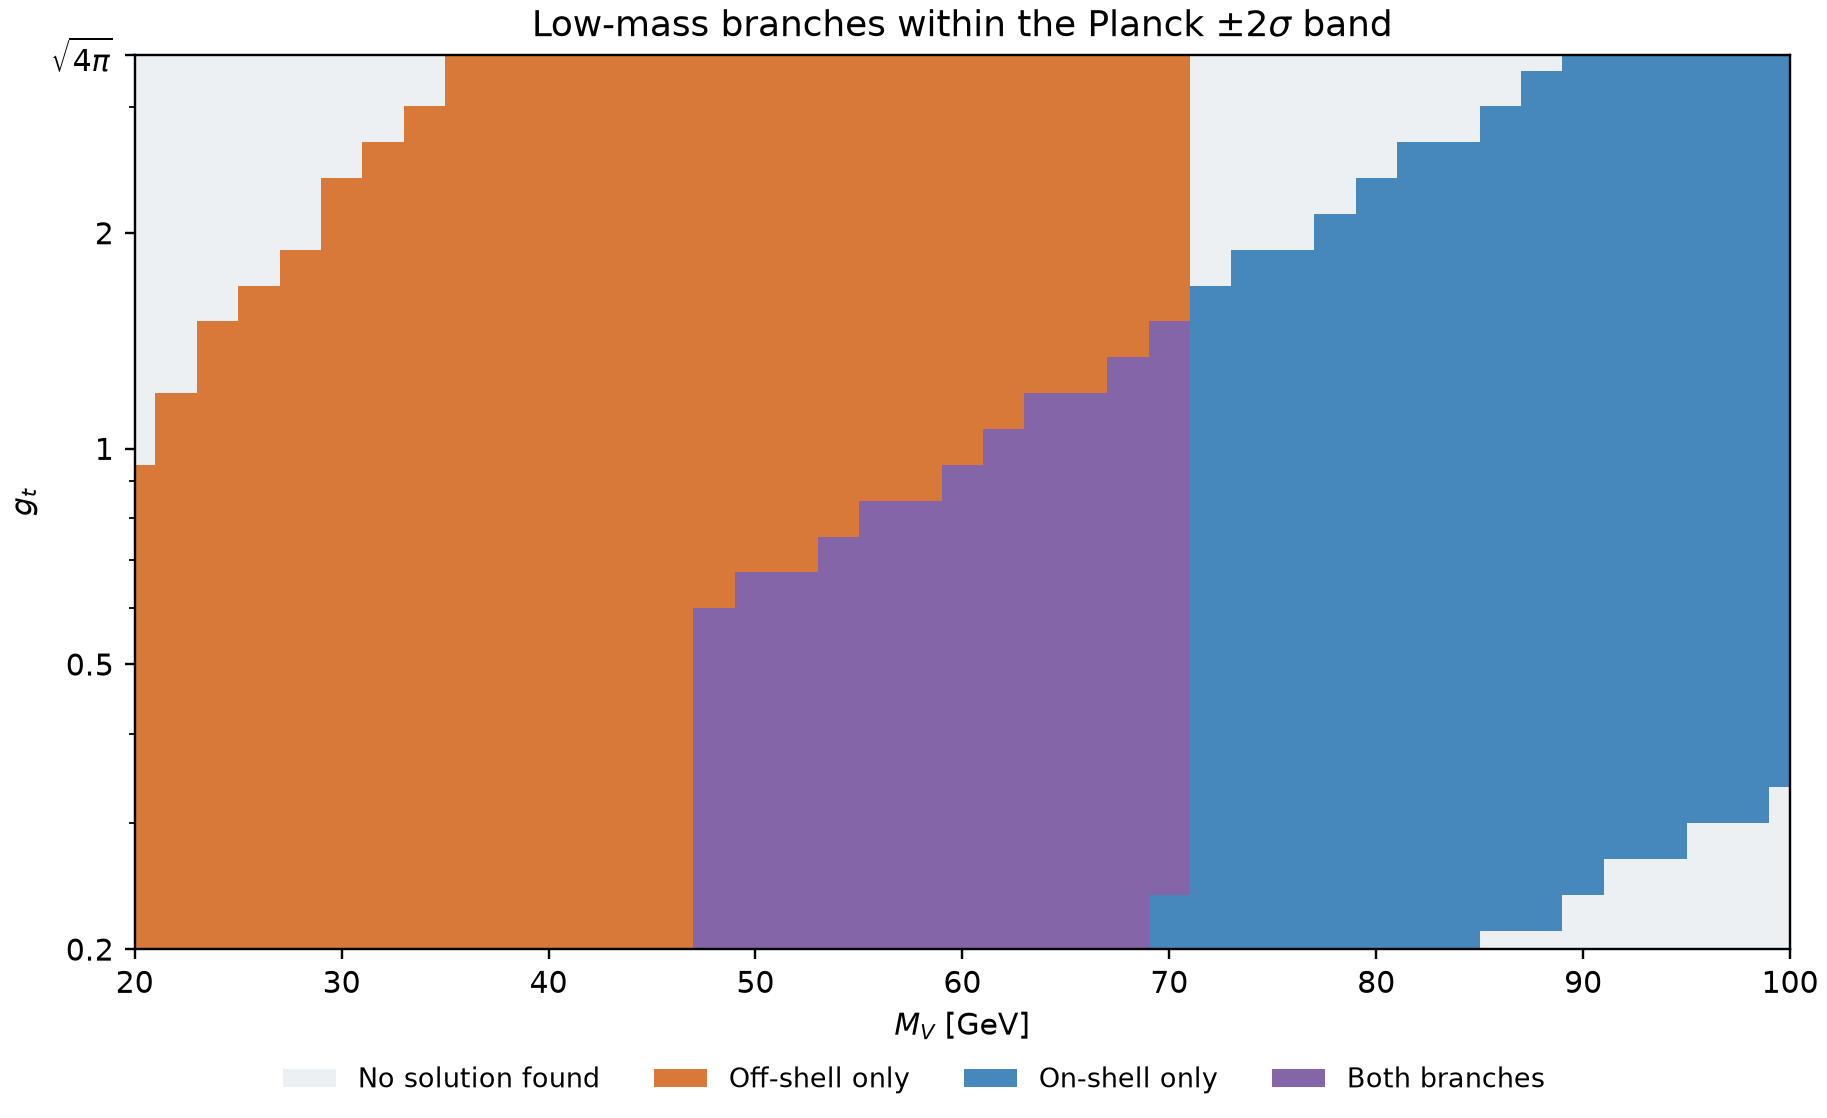
\includegraphics[width=\linewidth]{figures/d01_light_top_branches.png}
\caption{Independent low-mass scan with tree-level yield matching. Colors identify the relic branches found within the Planck $\pm2\sigma$ band. Purple indicates that both on-shell and off-shell solutions are present.}
\label{fig:low_mass}
\end{figure*}

The exploratory single-top calculation uses the 15-bin CMS AH $1b\,1\mathrm{FJ}$ projection with diagonal background uncertainties, truth cuts, simplified top decays, and approximate $b$ tagging. At $(M_V,g_t)=(60\,\mathrm{GeV},0.399)$, partonic-energy cuts $\sqrt{\hat s}<1.5,1.0,0.75$ TeV give median expected limits of 0.052, 0.337, and 3.43. This strong variation reflects the sensitivity of longitudinal charged-current amplitudes to electroweak cancellations with unequal top and bottom vector couplings. It limits the result to an exploratory estimate and is not used in the primary sensitivity map. \cite{kahlhoefer2016,cmstop,cmsahdata}

\begin{figure*}[tbp]
\centering
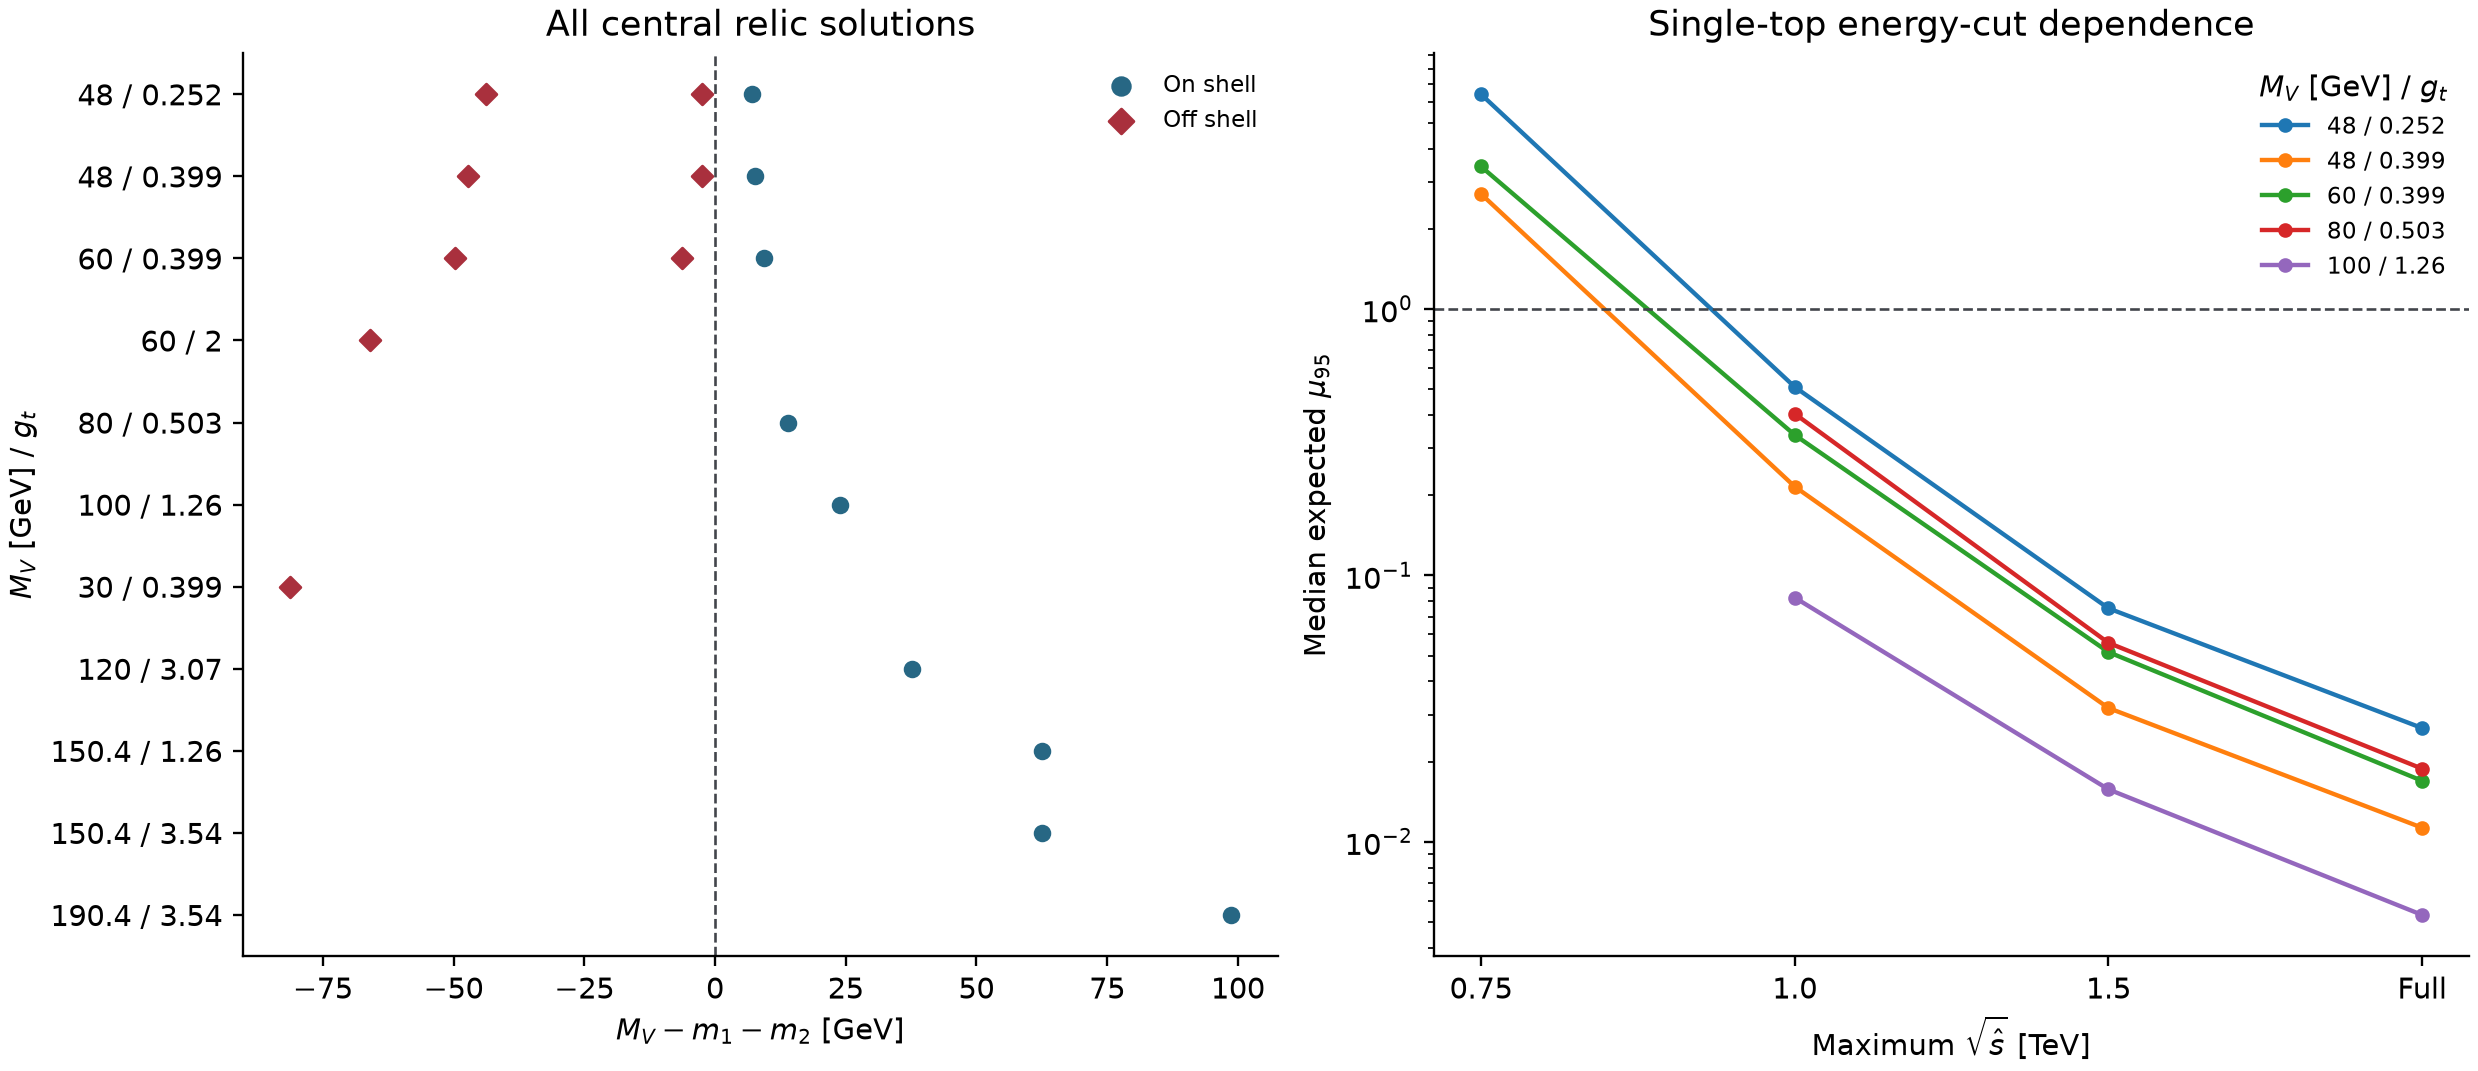
\includegraphics[width=\linewidth]{figures/08_top_branches_and_energy.png}
\caption{The left panel shows $M_V-m_1-m_2$ at representative central relic solutions. The right panel shows how the expected single-top sensitivity varies with the partonic-energy cut for on-shell solutions. The charged weak current connects top and bottom quarks with different $V$ couplings, so the high-energy behavior of longitudinal weak-boson amplitudes depends on cancellations in the electroweak completion. Varying the cut probes that dependence. Missing markers at 0.75 TeV indicate samples for which the approximate likelihood gives no finite limit.}
\label{fig:single_top_cut}
\end{figure*}
